The Square Root is quite complicated from a computational point of view; in fact, the most efficient known algorithms require to compute this operation by using an iterative approach, involving a chain of multiplications and other operations. The two most famous algorithms are the Newton-Raphson method and Goldschmidt’s algorithm. The latter has been chosen for bfloat16, since it's suitable for an efficient hardware implementation. 
\\
Given a Significand $S$, Goldschmidt's algorithm can be used to compute $\sqrt{S}$. With only one small variations, it's also possible to compute $\frac{1}{\sqrt{S}}$.\\
The objective is to find a series of $R_0$, $R_1$, ... , $R_n$ such that the following product tends to 1:
$$B_n = S*R_0^{2}*R_1^{2}* ... * R_{n-1}^{2} \approx 1 $$
Then, we can approximate the Square Root as:
$$ X_{n} = S * R_0*R_1* ... * R_n \approx \sqrt{S} $$
And the Inverse Square Root as:
$$ Y_n =   R_0*R_1* ... * R_n \approx  \frac{1}{\sqrt{S}}$$

Goldschmidt's algorithm initializes its variables as follow:

\begin{itemize}
\item $B_0$ = S
\item $Y_0$ = $R_0$ = $\frac{3-S}{2}$
\item $X_0$ = S * $R_0$
\end{itemize}

Each Goldschmidt's iteration firstly consists of computing:

\begin{enumerate}
\item $B_i$ = $B_{i-1}$ * $R_{i-1}^{2}$
\item $R_i$ = $\frac{3-B_i}{2}$
\end{enumerate}

And secondly it updates the Square Root and the Reciprocal Square Root approximations as follow:
\begin{enumerate}
\item $X_i$ = $X_{i-1}$ * $R_i$
\item $Y_i$ = $Y_{i-1}$ * $R_i$
\end{enumerate}

Iterations stop when R reaches a good approximation of 1.\\

We wanted to show that the Goldschmidt algorithm is very efficient, as it requires only a very small number of iterations to reach the desired precision. To do so, we quickly implemented the algorithm in Matlab and tracked the values of $B_i$, $R_i$, $Y_i$ and $X_i$ for ten iterations.\\ The code (\ref{fig:Matlab_Algorithm}) is simply the software implementation of the algorithm, and we run it twice; the first time, we put $S$ = 1,5625, which yelds an exact Square Root (\ref{fig:S_15625}).  The second time, we used $S$ = 1,5, which instead yelds an irrational number as solution (\ref{fig:S_15}).\\
In both cases, the algorithm converges in 5 or 6 iterations. Given that we only use 8 bits for the Mantissa, and not 24 like Matlab, we'll reach the desired precision in even fewer iterations.

\subsection{Additional notes}
In this section we presented only a quick and high-level description of Goldschmidt's algorithm. Implementation details were not discussed, but they are quite important. For example:
\begin{itemize}
\item Goldschmidt's algoritmh is not self-correcting, meaning we can't fully trust the LSB.
\item The values (significant included) are in the bfloat16 format, and must be consequently managed (e.g.: the value 3 used in the algorithm is represented as 9b'110000000).
\item The full square root algorithm requires also to compute the final exponent.
\end{itemize}
These and other details are more widely discussed in the next section.
\begin{figure}[h]
	\centering
	\captionsetup{justification=centering}
	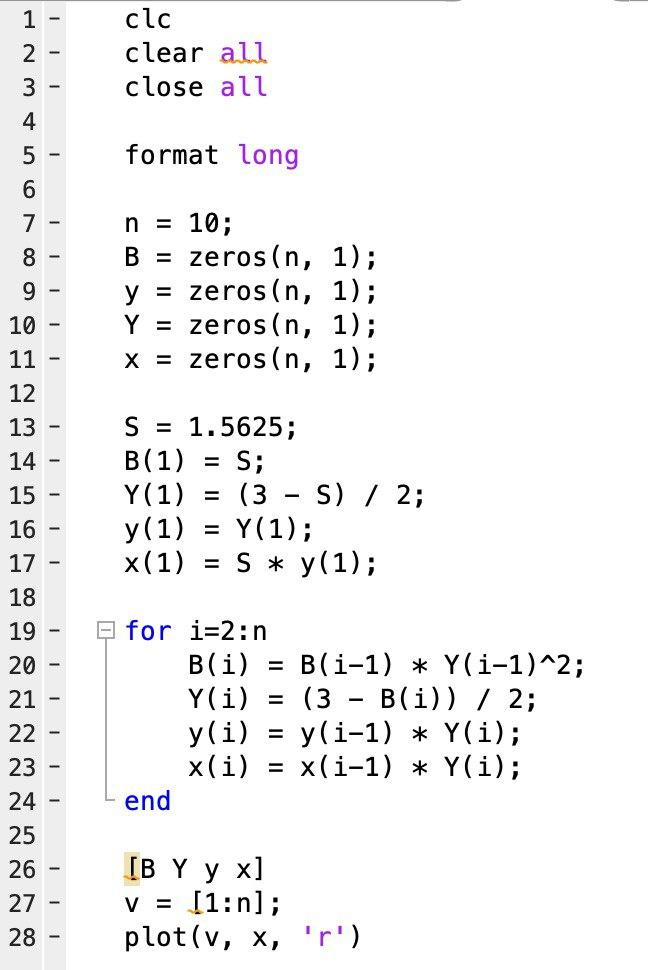
\includegraphics[scale=0.5]{Matlab_Algorithm.jpg}	
	\caption{Goldschmidt's algorithm implemented in Matlab}
	\label {fig:Matlab_Algorithm}
\end{figure}

\begin{figure}[h]
	\centering
	\captionsetup{justification=centering}
	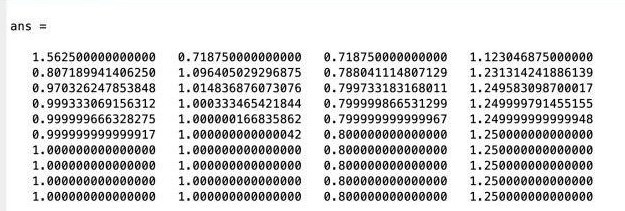
\includegraphics[scale=0.7]{S_15625.jpg}	
	\caption{Results with S = 1,5625\\From left to right, the values of B, R, Y, X}
	\label {fig:S_15625}
\end{figure}


\begin{figure}[h]
	\centering
	\captionsetup{justification=centering}
	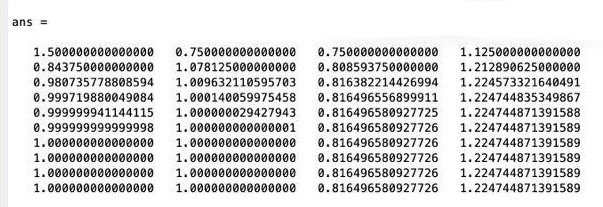
\includegraphics[scale=0.7]{S_15.jpg}	
	\caption{Results with S = 1,5\\From left to right, the values of B, R, Y, X}
	\label {fig:S_15}
\end{figure}

\clearpage
